\chapter{Evaluation}
\label{sec:evaluation}
% Analyse on expressions instead of statements.
% Statements that contain a block should have not been split as this makes reconstruction very difficult.
Evaluating the success of my solution is difficult. My implemented solution only works for some examples, as only some features of the language are supported. It focus is on parallelising as much as possible, not necessarily on getting a faster program. To get an idea of how much parallelism was found, the parallel source code was statically examined to find out how many threads and channels are created. These values may be lower than the actual number of threads used, as some thread definitions will be reused (repeated function call, for loops, etc.). Each program was compiled sequentially and in parallel, without and with optimisations.

Two manually written sequential programs were parallelised: a simple example and a password cracker. The dependency tree and schedule are analysed to show how the parallelising compiler works. To test the robustness of the compiler, a collection of automatically generated sequential programs were also parallelised. The output of the parallel version was compared with the sequential version to check that the parallelisms have not semantically changed the program.

\section{Sequential Programs Parallelised}
\subsection{Simple Example}
This simple example is intended to be an easy way to show how the parallelising compiler works. It consists of two independent variables, \texttt{a} and \texttt{b} which are incremented and then printed together. An extra independent print statement is also added at the end to show one potential problem with the dependency analysis.

\begin{code}
    \inputcode{simple-example/main.rs}{}{}
    \caption{A simple example program}
\end{code}

\begin{figure}
    \begin{subfigure}{.5\textwidth}
        \centering
        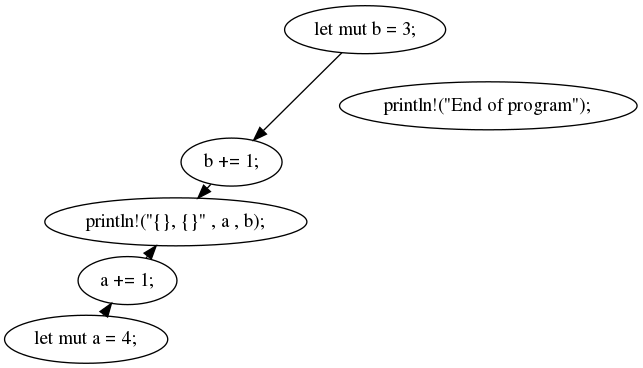
\includegraphics[width=\textwidth]{img/simple-example/main-dependency-analysis.png}
        \caption{\label{fig:simple-deps}Dependency analysis}
    \end{subfigure}
    \begin{subfigure}{.5\textwidth}
        \centering
        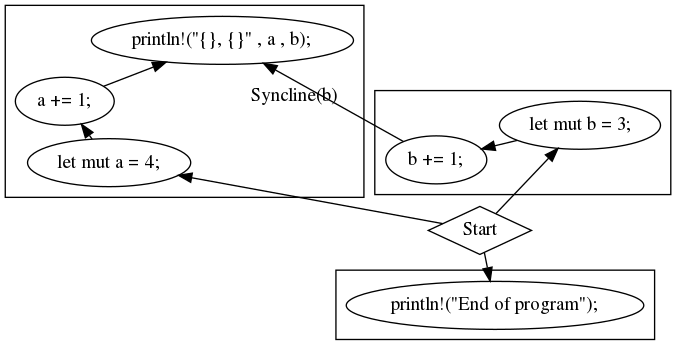
\includegraphics[width=\textwidth]{img/simple-example/main-schedule.png}
        \caption{\label{fig:simple-sch}Schedule}
    \end{subfigure}
    \caption{Main method from the simple example program}
\end{figure}

\autoref{fig:simple-deps} clearly shows \texttt{a} and \texttt{b} do not need to be inter-weaved. It also shows that the \texttt{println!(``End of program");} is completely independent of the other print statement. This may not be intended by the programmer, but there is nothing inside the \texttt{println!} macro which states that they must be called in order (there is no variable linking the two print statements). This could be fixed by forcing non-analysed functions to be executed in order, but it may not be an actual dependency and it would reduce the number of parallelisms detected. Because this dependency is not detected, I sorted the outputs of both sequential and parallel programs so that the order does not matter when comparing program outputs. \autoref{fig:simple-sch} shows that the scheduling algorithm split \texttt{a} and \texttt{b} into separate threads as well as the ``End of program" print statement. The print statement that prints \texttt{a} and \texttt{b} attached itself to the \texttt{a} thread. The \texttt{b} variable is sent along the syncline just before the print.

\subsection{Password Cracker}
A password cracker program is a good target for paralleling. Each word in a dictionary is hashed individually and then compared with the hash of a password that the user is trying to crack. My implementation contains three functions: \texttt{loadDictionary()}, \texttt{hash()} and \texttt{main()}. The \texttt{loadDictionary()} is not analysed here as the parallelising compiler did not make any changes to this function. This program is on the limits of what my parallelising compiler can do in its current state. Some of the code is written in a semi-specific way to get it to parallelise properly.

\subsubsection{Hash Function}
The word argument is iteratively hashed $1000$ times with SHA256 from an external crate. If I let the parallelising compiler try to parallelise this loop, it would produce code that does not compile.
\texttt{hasher.result\_str()} returns a \texttt{str} which is normally converted to a \texttt{String}. When run in parallel, it tries to send a \texttt{str} down a syncline which does not work as \texttt{str} does not implement the \texttt{Send} trait.
This could be fixed by storing the type with the variable name instead of relying on type inference. Another reason for disabling parallelisation of this loop is that it would slow the program down. Most of the statements depend on the previous iteration and so no speedup can be achieved here. Line $32$ has no dependencies and could be be run in parallel but it is not computationally expensive to call \texttt{Sha256::new()} so it is not worth it. If some performance analysis technique was implemented, then it would notice that it is a bad idea to parallelise this loop.
To disable parallelisation of this loop, I added \texttt{.rev()} to the range. %(a little hacky)

\begin{code}
    \inputcode{password-cracker/main.rs}{27}{37}
    \caption{Hash function of the password cracker program}
\end{code}

\begin{figure}
    \begin{subfigure}{0.6\textwidth}
        \centering
        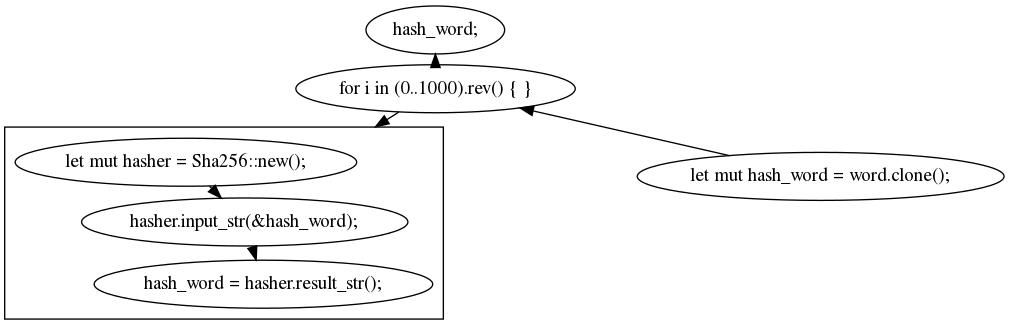
\includegraphics[width=\textwidth]{img/password-cracker/hash-dependency-analysis.png}
        \caption{\label{fig:hash-deps}Dependency analysis}
    \end{subfigure}
    \begin{subfigure}{0.4\textwidth}
        \centering
        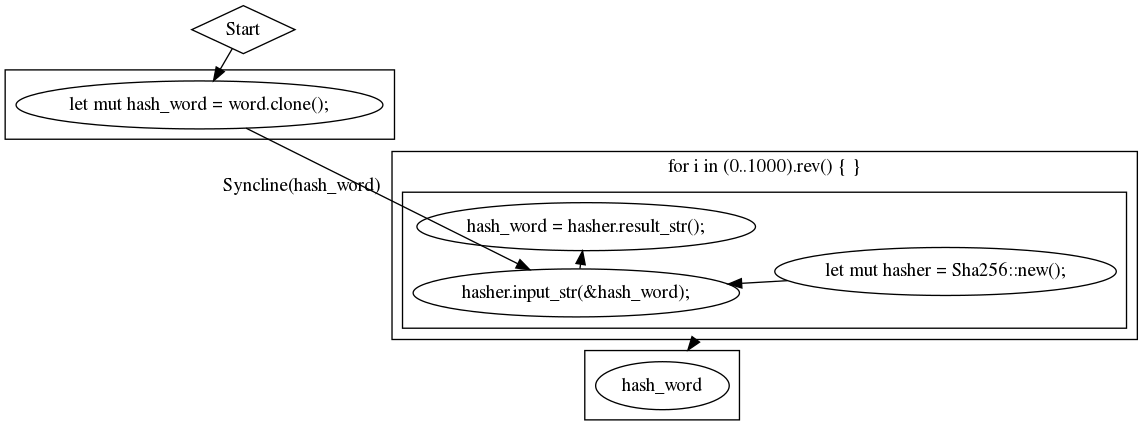
\includegraphics[width=\textwidth]{img/password-cracker/hash-schedule.png}
        \caption{Schedule}
    \end{subfigure}
    \caption{\label{fig:hash-sch}Hash function from the password cracker program}
\end{figure}

\autoref{fig:hash-deps} shows how the inner block is linear for one iteration. The reason that the loop cannot be parallelised effectively is that \texttt{hash\_word} is modified each iteration.
\autoref{fig:hash-sch} shows how linear the iterative hash function is. The only thread separate thread that is spawned clones the word. The reason that the for loop is not inside the same thread is because the \texttt{hash\_word} dependency is inside the for loop. The condition on the for loop is independent and could be slow and so is parallelised. In reality, this will be much slower due to thread overhead.

\subsubsection{Main Method}
The main method loads the dictionary from a file into a list of strings. Each word in this list is hashed and compared with a password hash. Notice that the for loop is not interrupted when it finds the correct word, or even stored; it is just printed. A timing circuit is placed around the function to print how long it takes to find the password.

\begin{code}
    \inputcode{password-cracker/main.rs}{39}{57}
    \caption{Main method of the password cracker program}
\end{code}

As you can see from the \autoref{fig:pass-deps} and \autoref{fig:pass-sch}, the timing circuit is a completely independent program. This is probably not intended, and it is a similar problem to the \texttt{println!} problem from the simple example. This is slightly different as the order for the time circuit is actually correct but the time that the timing circuit is run is different. There is no real fix I can think of for this issue except hard coding the time crate to be dependent on everything before it and everything after it dependent on it. I am not a fan of hard coding this, as there may be other functions in other crates which also have similar dependency requirements. I will just remove the timing circuit when comparing the outputs as the time will not be consistent between runs.
The schedule (\autoref{fig:pass-sch}) shows that the \texttt{password\_hash} assignment is placed in its own thread, as the for loop condition is independent. The block inside the for loop does depend on this value, and so a syncline is setup. It is not clear from the schedule above, but the for loop is also parallelised. \autoref{fig:pass-for-sch} shows how the each iteration of the for loop is parallelised and what synclines are required.
The \texttt{dictionary} and \texttt{password\_hash} variables are requested on the first line they are required in the iteration and sent to the next iteration when they are no longer needed. In this case, only one statement uses each external dependency, so it is immediately released. The \texttt{hash} function is computationally expensive, and can only be started once it has access to its word in the dictionary. The dictionary can be passed very quickly through all of the threads, as accessing the element inside a list is very fast. This allows multiple \texttt{hash} functions to be run at the same time. The \texttt{password\_hash} variable is requested after the \texttt{hash} function returns, meaning \texttt{id=1} cannot check whether it is equal to the \texttt{password\_hash} if its \texttt{hash} function returns before \texttt{id=0}.

\begin{figure}
    \begin{subfigure}{\textwidth}
        \centering
        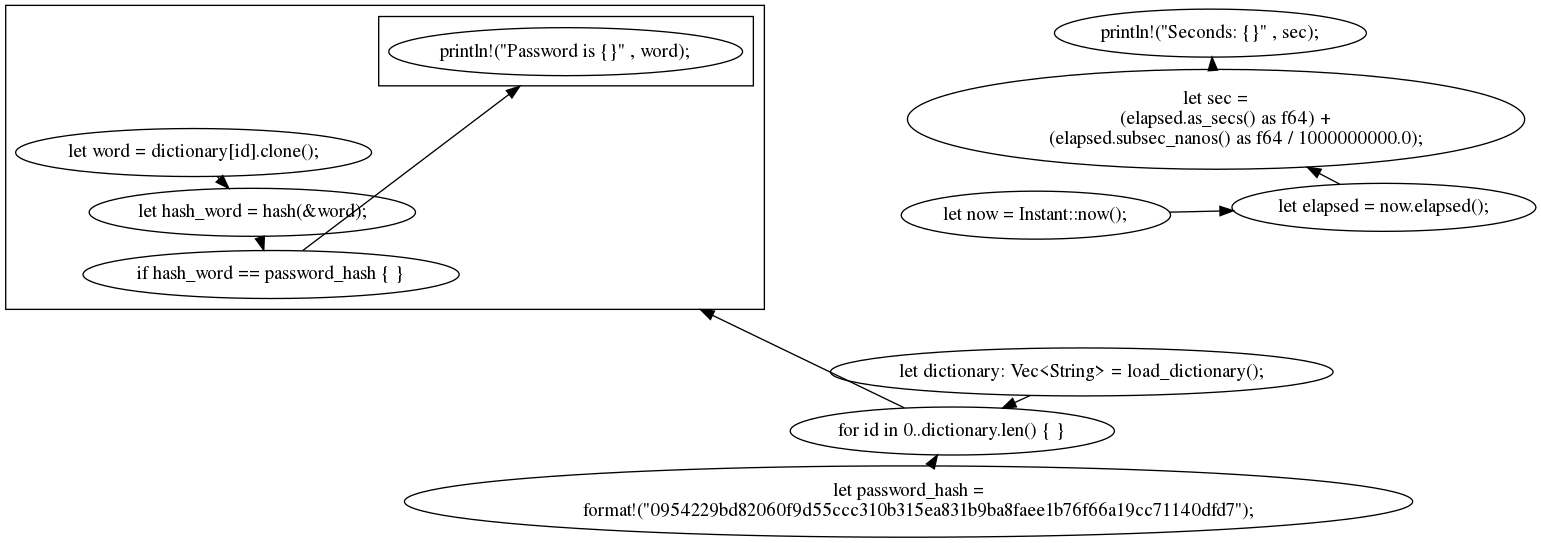
\includegraphics[width=\textwidth]{img/password-cracker/main-dependency-analysis.png}
        \caption{\label{fig:pass-deps}Dependency analysis}
        \vspace{1em}
    \end{subfigure}
    \begin{subfigure}{\textwidth}
        \centering
        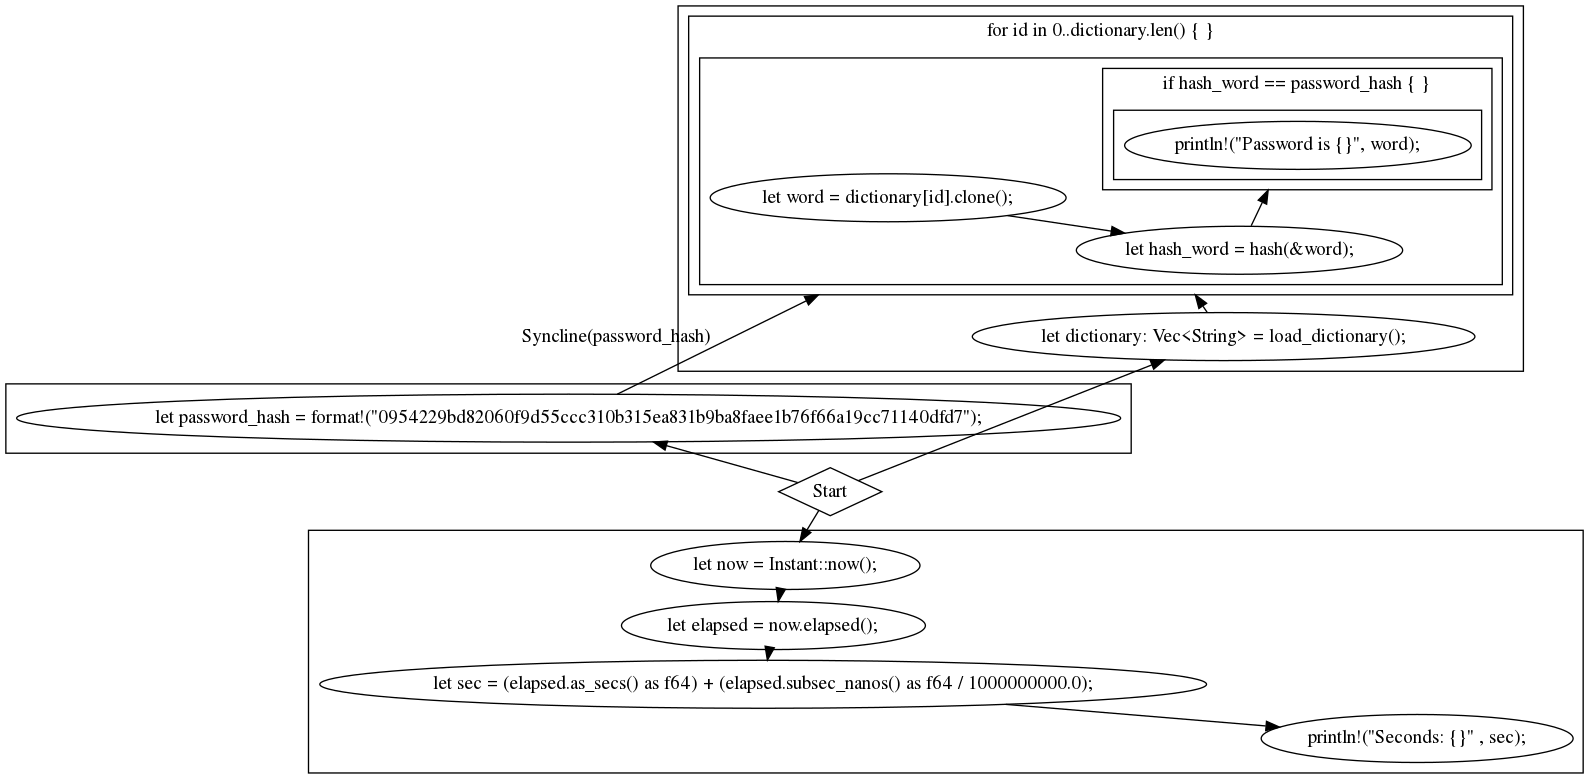
\includegraphics[width=\textwidth]{img/password-cracker/main-schedule.png}
        \caption{\label{fig:pass-sch}Schedule}
    \end{subfigure}
    \caption{Main method from the password cracker program}
\end{figure}

\begin{figure}[H]
    \centering
    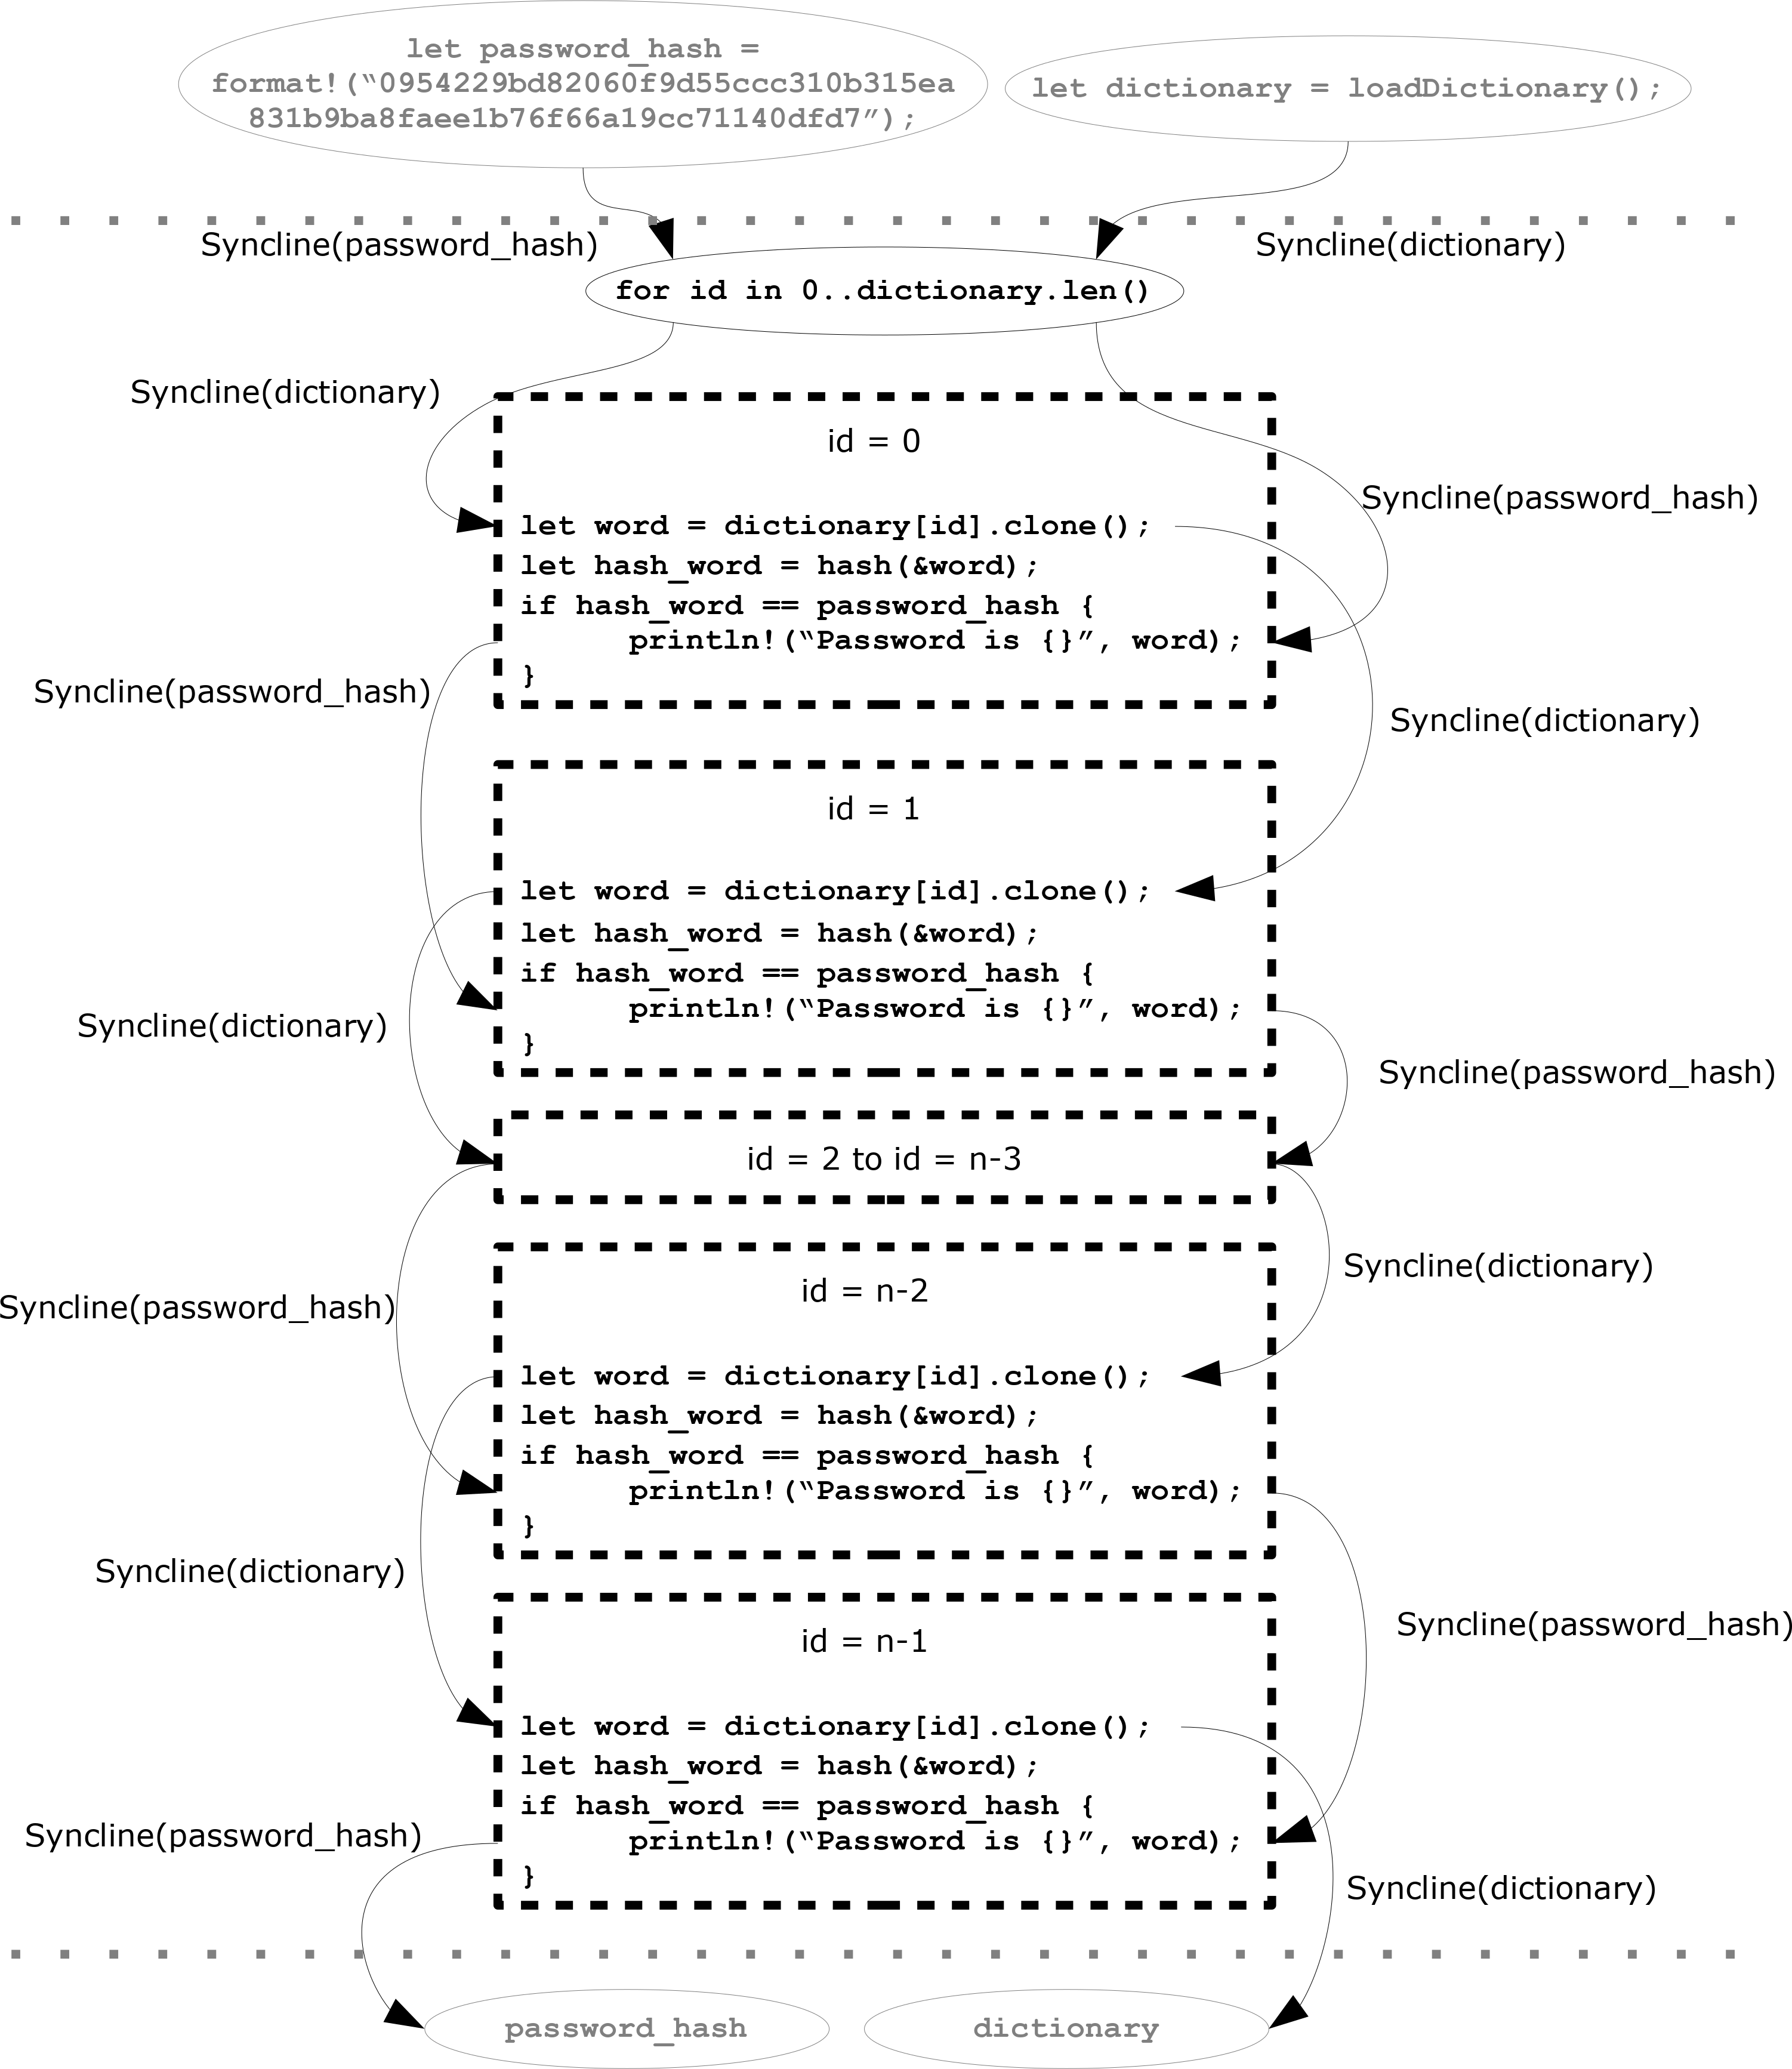
\includegraphics[width=\textwidth]{img/password-cracker/parallel-for.png}
    \caption{\label{fig:pass-for-sch}A schedule to show how the for loop in the main method from the password cracker program is parallelised}
\end{figure}

\subsection{Automatically Generated Sequential Programs}
\todo{PROOF READ UP TO HERE}

To verify that the parallelising compiler can parallelise more that the programs shown above, it was tested against $1428$ randomly generated sequential programs. Each randomly generated sequential program was executed sequentially and in parallel, with and without compiler optimisations to compare the outputs. This is to verify that the program semantics remains the same. The sequential and parallel program was run $1000$ times, and their execution time was recorded. The number of concurrent threads executed was also recorded for the parallel program. I am not expecting a speedup in the parallel programs as the size of the problem remained fairly small, and is probably not enough to overcome the thread overhead. The more interesting value will be the number of concurrent threads executed, as this shows how much parallelism the parallelising compiler could find in the sequential program. It gives us a gauge on how fast the parallel version could be if there was no thread overhead.

\todo{Show example of a randomly generated program?}

\section{Results}
\todo{Include results from simple example}

\todo{Include results from password-cracker}

\todo{Include results from automated testing}
